\documentclass[10pt,a4paper]{article}
\usepackage[utf8]{inputenc}
\usepackage{url}
\usepackage[english]{babel}
\usepackage{amsmath}
\usepackage{amsfonts}
\usepackage{amssymb}
 \usepackage{float}
\usepackage{graphicx}
\usepackage[left=2cm,right=2cm,top=2cm,bottom=2cm]{geometry}
\author{Andres Chaves}
\title{Research Proposal}

\begin{document}
 \title{Research Proposal}
 \author{Andres Chaves (706801) \\
  \multicolumn{1}{p{.7\textwidth}}{\centering{achaves@student.unimelb.edu.au\\}\centering\emph{Melbourne School of Information\\The University of Melbourne}}}
 \maketitle

\begin{abstract}
    The purpose of this document is to establish the context and basis of my research project, which applies concepts of Machine Learning into Network Management Systems.
   \\\\
   Throughout this document we will read the relevance of the research, how will the concepts of Machine Learning will be applied to Event-processing Network Management Systems and finally what are the expected results.
\end{abstract}


\tableofcontents

\newpage
 \section{Introduction}
 There is no doubt on the strong development and evolution of information technologies in the modern world. Nowadays, we have access to computing devices in several forms such as supercomputers, laptops, tablets and smart phones; and of course this device evolution comes in conjunction with advances in distributed information systems.
 \\\\
 But this evolution could not be accomplished without a key component: computer networks. Networks allow data exchange and information services consumption possible and side by side with information technology, it has evolved from simple small low bandwidth networks to high speed wired and wireless ones connecting all the world.
 \\\\
 These huge networks require a set of practices, tools and knowledge in order to guarantee the availability and quality of service required by clients. A discipline called Network Management has arisen to address all these previous concerns and nowadays Network Management comprises all the practices and activities that a carrier must perform in order to fulfill its Service Level Agreements (SLAs) with its clients.
 \\\\
 From the information systems perspective, Network Management requires a set of systems called Network Management Systems (NMS), designed to administer either all or a part of the network. This administration is composed by a set of functions: Fault Management, Performance Management, Configuration Management and Security Management among others.
 \\\\
 Fault Management involves how to detect, classify and inform network operators about conditions that affect or may affect the network services, both from availability and performance perspective. Typically, network elements inform this to an  information system in an asynchronous way using SNMP protocol, specifically a SNMP TRAP event.
 \\\\
 One of the challenges in Network Management is how to monitor ever bigger networks where there are network devices in the range of thousands to millions. With a network of this size, the rate of alarms received by a system can be around hundreds of events per second and with this alarm ratio a key desired function of a NMS is to only show the relevant alarms to the network operators.
 \\\\
 One possible approach to analyse, classify and display only the relevant events to the operator is by the use of a machine learning system that helps the network operator to process events and thus augment the network management capacity with the same engineering team size.
 \\\\
 This project intends to advance in this approach by formulating an strategy and measuring the improvement, from a fault management perspective, of its implementation.

 \section{Objective}
The objective of this project is to analyse how machine learning technologies can be applied to Network Management Systems, specifically event/fault management systems in order to reduce the alarm rate and report only key events to the network operators and thus increase the network management capacity of a Network Operation Center.
\\\\
The Machine Learning technique will be used to reduce the volume of alarms by suppressing correlated or secondary alarms for a given network event. With this approach we do not intend to replace the judge and knowledge of the engineer but quickly 
help him/her in discovering what correlation rules may be applied to reduce the alarm ratio.

  \section{Problem Definition}
A Fault Management System (FMS) is a stream processor of alarms where they are received, processed and displayed:

\begin{figure}[H]
 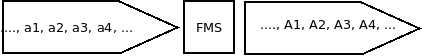
\includegraphics[scale=0.4]{NMS_FMS.png}
  \centering
  \caption{\textit{An abstraction of a Fault Management System}}
  \label{fig:nms_fms}
\end{figure}	

Whenever a relevant event happens on a network, each network element sends alarms according to their role. A network event is translated into several alarms that may come from different sources. For example, if the event is a physical medium failure, the transmission TX equipment will send an alarm reporting this, but also all the networks elements that rely on this medium will perceive the event. For example, if a Switch equipment is related to the TX equipment then it will send a Layer 2 alarm and also a if Router is connected then a Layer 3 alarm will be sent. We can see that a network event is translated into a cascade of different events and therefore, given an event E1 the FMS system may receive several alarms from different network elements:
\\\\
\begin{figure}[H]
 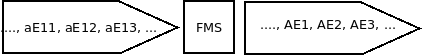
\includegraphics[scale=0.4]{NMS_FMS_EVENT.png}
  \centering
  \caption{\textit{A representation of the alarms of a given event arriving to a FMS}}
  \label{fig:nms_fms_event}
\end{figure}	

It is important to mention that several events can be happening at the same time in a network and thus the FMS receives a storm of alarms from different sources and that also the alarms can be received in different order. The FMS is a system built to recognize alarms but is unable to identify which alarms belong to the same event:
\\\\
\begin{figure}[H]
 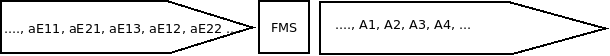
\includegraphics[scale=0.4]{NMS_FMS_EVENTS.png}
  \centering
  \caption{\textit{Several alarms from different events arriving to a FMS}}
  \label{fig:nms_fms_events}
\end{figure}	

Because the FMS is unable to recognize which alarms are related to the same event the volume of alarms presented to the network operator is dramatically high. In this sense, we require a component in the FMS that allows the system to infer what alarms are related to the same event and then suppresses them, showing only one single alarm. However, it would be impractical to explicitly develop this component due to the number of different events present in a network, the number of possible alarms and the time required from the expert to analyze the relation between events and alarms.


  \section{Proposed Solution}

Given that the development of a correlation component might be impractical, a machine learning system is proposed to address the implementation of this required functionality. A common definition of a machine learning system is a computer system that can perform a function without being explicitly programmed \cite{mlsamuel}. In this sense, we want a machine learning system as a component of the FMS which allows the system to infer what alarms are related to the same event and then suppress them, showing only one single alarm. 
\\\\
More formally, we can represent our desired Machine Learning System outcome as a function \textit{h} that receives the input stream of alarms and classifies whether the alarms are related to the same event:

\begin{figure}[H]
 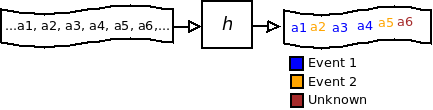
\includegraphics[scale=0.4]{MLS_hypothesis.png}
  \centering
  \caption{\textit{Representation of the proposed Machine Learning System}}
  \label{fig:mls_hypothesis}
\end{figure}	

Note that the system is not interested in knowing what is the specific type of event but whether the alarms belong to the same event, whichever it is.
\\\\
In order to generate this function \textit{h}, the learning algorithm needs an input training set from which the algorithm will fit the function.
\\\\
Depending on the characteristics of the training set we define the technique of machine learning. In supervised learning the training set is previously labeled, separating the true examples from the false ones. The learning algorithm fits the function by generalizing the examples and establishing a function that separates the examples or in other words classifies them.
\\\\
Conversely, in unsupervised learning the training set comes without a previous labeling and it is the job of the machine learning algorithm to try to find groups or classify the examples without the initial set of classified input.
\\\\
The proposed solution will use a semi-supervised technique. In semi-supervised learning some examples from the training set are labeled but the majority are not\cite{mlInNetworking}. Specifically, the network operator will label one alarm that he considers represent an event.
\\\\
Given this labeled example, the system will generate a training set from the historical set of alarms where the labeled alarm is present, and this is the training set that will be used with an unsupervised learning algorithm. The outcome of the machine learning algorithm will be a classifier for the alarms.
\\\\
This classifier is presented to the network operator which confirms if the correlation is correct and therefore the classifying rules are incorporated into the Fault Management System by classifying and suppressing future alarms concerning the labeled alarm.
\\\\
A conceptual scheme of the proposed solution can be seen on Figure \ref{fig:proposed_solution}

\begin{figure}[H]
 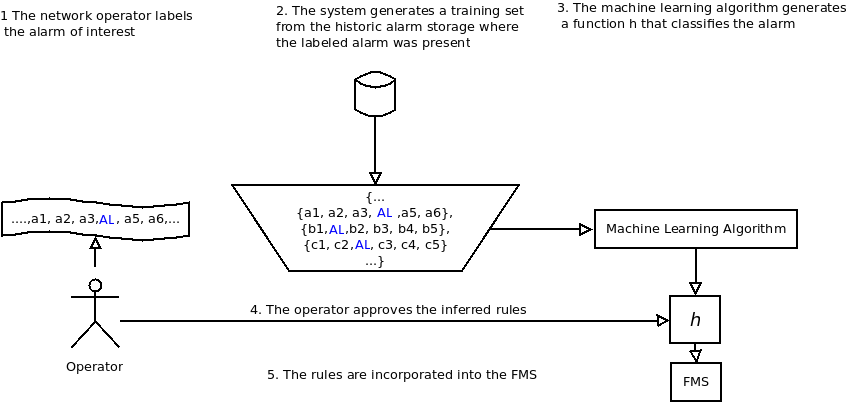
\includegraphics[scale=0.4]{proposed_solution.png}
  \centering
  \caption{\textit{A schematic of the proposed solution}}
  \label{fig:proposed_solution}
\end{figure}	


  \section{Technical Details}
A generic SNMP Fault Management System is a stream based system that conceptually can be divided into several stages: Alarm reception, alarm translation and enrichment, event correlation and event presentation. A conceptual schema can be seen on Figure \ref{fig:nms_generaldiagram}
\\\
\begin{figure}[H]
 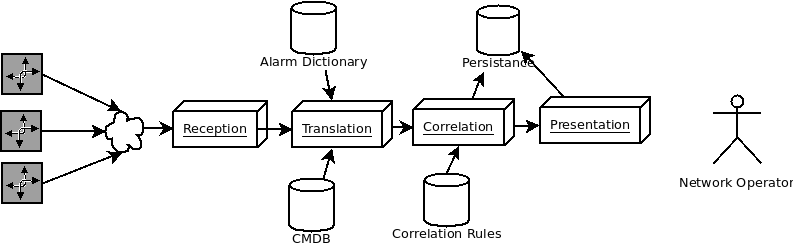
\includegraphics[scale=0.4]{NMS_GeneralDiagram.png}
  \centering
  \caption{\textit{A schematic of a generic Network Management System}}
  \label{fig:nms_generaldiagram}
\end{figure}	

For our testing environment we are going to use several components to simulate a Fault Management System. These are described as follows:

\begin{itemize}
  \item Net-SNMP: Net-SNMP is an open source Linux and Unix package that implements the SNMP protocol. The role of this component will be the reception of alarms\cite{netsnmp}
  \item SNMPTT: SNMPTT or SNMP-Trap Translator is an open source component that takes the SNMP trap (alarm) received by Net-SNMP and by using an alarm dictionary translates it into a more useful event. SNMPTT can also enrich the alarm from a database by executing a shell script.\cite{snmptt}
  \item MLS: The Machine Learning System component will apply the correlation function generated by our learning algorithm.\cite{sec}
  \item MYSQL: MySQL is an open source relational database. For this project, it will be used as storage of the Alarms and Configuration Management Database.
  \item Frontend: There will be a frontend to show the reduced alarms to network operators.
\end{itemize}


  \section{Time Table and Deliverables}
The research project is decomposed by the following tasks and deliverables:

\begin{center}
 \begin{tabular}{||c | c | c | c||} 
 \hline
 Task & Date & Deliverable \\ [0.7ex] 
 \hline\hline
 First version of Research Proposal  & 2015/03/02 & Yes \\ 
 \hline
 Initial Data Set Acquisition (without Classification) & 2015/03/02 & No \\ 
 \hline
 Establishing ML Techniques to be used & 2015/03/13 & No \\
 \hline
 Development of a quick prototype to label alarms & 2015/03/27 & No \\
 \hline
 Result Acquisition and Analysis  & 2015/04/17 & No \\
 \hline
 First version of the final report (Thesis) & 2015/05/01 & Yes \\
 \hline
 Final version of the final report (Thesis) & 2015/05/29 & Yes \\

 \hline
\end{tabular}
\end{center}

  \section{Expected Results}

It is expected that the rules inferred from the Machine Learning System are useful, accurate and general as possible in order to present only key events to Network Operators. Also it is expected a comparison between the different techniques tested.
\\\\
Normally, carriers buy expensive Network Management Systems, with correlation capabilities, but the lack of time or knowledge from Network Operators causes to not take advantage of these powerful tools. With this approach, a set of rules can be generated and quickly incorporated into a Network Management System increasing its value added to the process of Network Management.

  \section{Literature Review}
As Network Management involves processing and analysis of large datasets there has been several attempts to use Machine Learning techniques to aid or improve this large analysis.
\\\\
The majority if the reviewed literature attempts to use Machine Learning into traffic flow analysis and Security. Traffic Analysis is one of the key parts in Network Management because it allows to determine patterns and behaviour segmented by type of traffic (HTTP, FTP, P2P, etc). For the security part the intention is to use Machine Learning to aid in the analysis of security logs to detect intrusion or attacks. While these topics are also part of Network Management the objectives and results differ with the purpose of this research.
\\\\
There are a couple of papers that have explored how to apply Machine Learning to alarm handling, The first one titled "Algorithm of Mining Fuzzy Association Rules in Network Management" attempts to reduce the volume of alarms in a event database by applying the theory of Fuzzy Sets to find the frequent sets and association rules between them.\cite{liu2003}.
\\\\
The second one, named "An Artificial Intelligence Approach to Network Fault Management" discuss what Artificial Intelligence methods can be applied to fault management and suggest the use of either Neural Networks or Bayesian Belief Networks to the problem \cite{kefferundef}.

\newpage

\begin{thebibliography}{9}

\bibitem{mlsamuel} A. L. Samuel,
        \emph{Some studies in machine learning using the game of checkers}.
        IBM Journal of Research and Development, 3(3):210–229, July 1959. ISSN 0018-8646
\bibitem{mlInNetworking}Understanding Network Traffic, An Introduction to Machine Learning in Networking,  \url{http://www.tma-portal.eu/wp-content/uploads/2011/12/TMA_phd_Machine_Learning.pdf}.
\bibitem{netsnmp}Net-SNMP website, \url{http://www.net-snmp.org/}.
\bibitem{snmptt}SNMPTT website, \url{http://snmptt.sourceforge.net/docs/snmptt.shtml}.
\bibitem{sec}SEC website, \url{http://simple-evcorr.sourceforge.net}.
\bibitem{liu2003}
  Pei-Qi Liu, Zeng-Zhi Li, Yim-Liang Zhao,
  \emph{Algorithm of Mining Fuzzy Association Rules in Network Management}.
  Proceedings of the Second International Conference on Machine Learning and Cybernetics, Xi'an,
  2003.
\bibitem{kefferundef}
  Denise W. Gürer, Irfan Khan, Richard Ogier, Renee Keffer,
  \emph{An Artificial Intelligence Approach to Network Fault Management}.
  
\end{thebibliography}
    
\end{document}